\section{\name Overview}\label{s:design}
\begin{figure*}
    \centering
    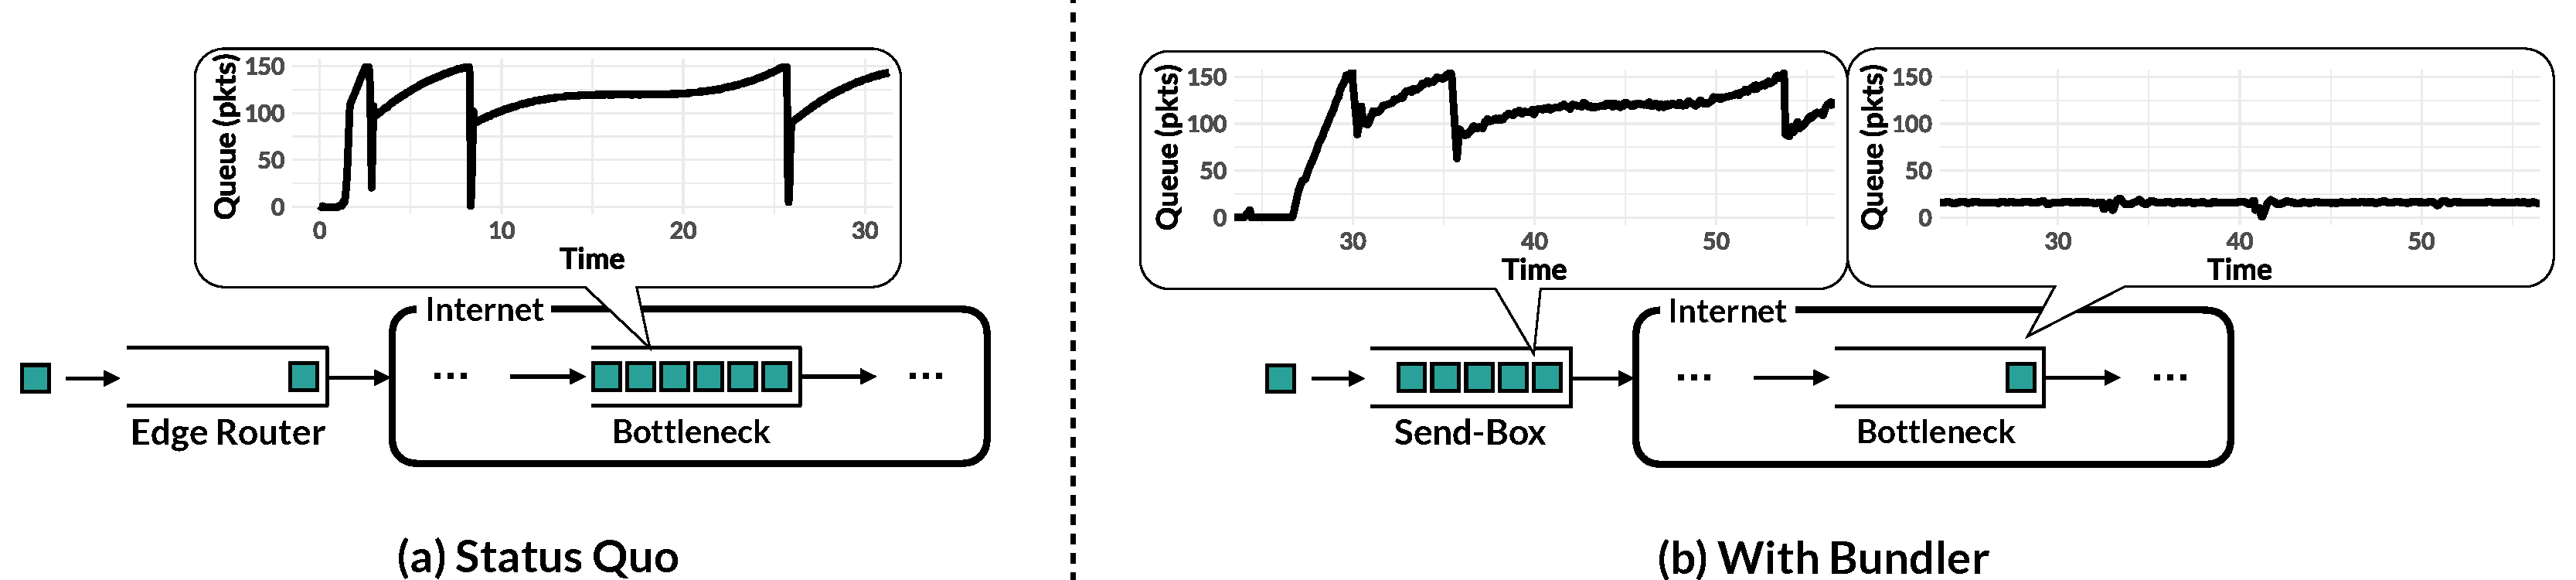
\includegraphics[width=\textwidth]{img/shift-bottleneck-combined}
    \caption{This illustrative example with a single flow shows how \name can take control of queues in the network. The bubbles show the trend in measured queueing delays at the relevant queue over time. The queue where delays build up can best make scheduling decisions, since that is where there is the most choice between packets to send. Therefore, the \inbox \emph{shifts} the queues to itself to gain scheduling power.}\label{fig:design:shift-bottleneck}
\end{figure*}

\cut{
A \name must have the following properties:
\cut{ 
% these items could be considered implementation details
    \item It measures congestion control information from the network path.
    \item It enforces a pacing rate determined by a congestion control algorithm. The congestion control algorithm takes as input measurements from the network path, and returns an aggregate rate at which \name should send its component traffic.
}
\fc{mabye this starts too abruptly}
\begin{enumerate}
    \item It provides a mechanism for scheduling the packets comprising the aggregate.
    \item It must be deployable, therefore, it cannot rely on changes in end-hosts.
    \item It must be capable of deployments on the edge of a domain. Therefore, it must also scale to high link rates. As a result, it should not maintain per-connection state -- only per-aggregate state. \radhika{shorten}
\end{enumerate}
\radhika{Need a transition line: ``The rest of this section discusses .....''} 
}

%\subsection{Shifting the Queues}\label{s:design:shifting}

%The key insight of \name is that shifting the queues induced by a traffic bundle from the bottleneck to the sender's edge enables the sender to schedule the traffic within the bundle appropriately. Notice that \name can only shift (and therefore can only schedule) the component of the bottleneck queue which is self-inflicted by the traffic in a given bundle. 

A trivial strategy for inducing queuing at the \name, to effectively schedule the flows within a bundle, is to throttle its outgoing rate. However, if this rate is made smaller than the bundle's share of bandwidth at the bottleneck link, it can adversely affect its throughput. Instead, the rate needs to be set such that bottleneck link sees a small queue while remaining fully utilized (and such that the bundled traffic competes fairly in the presence of cross traffic). We make a simple, but powerful, observation: some existing congestion control algorithms~\cite{nimbus, copa} perform exactly this calculation. Therefore, running such an algorithm at the \name to set a bundle's rate, would reduce its self-inflicted queueing at the in-network bottleneck, and shift it to the \name instead, without impacting the bundle's aggregate throughput. 
%In order to prevent under-utilization of the bottleneck links in the network, \name needs to occupy . 
%We make a simple, but powerful, observation: many congestion control algorithms perform exactly this calculation! 
%If we run an appropriate congestion control algorithm (as discussed later in \S\ref{s:design-choices}) at the \name, it will decide on a fair sending rate for each of its bundles as they compete with traffic from other domains. 
%Component flows of the bundles will then queue at the \name as their packets are sent at this rate.
%Since component flows, running traditional congestion control algorithms, will probe for bandwidth until they experience loss, they build queues at the \name instead of at the bottleneck.
%Since the \name now controls the queues corresponding to the traffic aggregate, it can schedule the packets of component flows. \radhika{needs fixing!}

Figure~\ref{fig:design:shift-bottleneck} illustrates this method for a single flow traversing a bottleneck link in the network.\footnote{Details of the emulated network setup which resulted in the illustrated queue length time-series has been provided in \S\ref{s:eval}.} In Figure~\ref{fig:design:shift-bottleneck:before}, packets from the endhosts are queued in the network, while the queue at the edge is unoccupied. In contrast, in Figure~\ref{fig:design:shift-bottleneck:after}, the \name deployed at the edge (and implementated as described in \S\ref{s:impl}) is able maintain very low queuing at the bottleneck by using a congestion control algorithm to compute and send at the bottleneck rate.

%In the remainder of this section, we describe our design requirement and choices for \name. 
\radhika{transition line}

\Para{Key properties} Our design choices, guided by our key requirement of \emph{deployment and management ease}, resulted in the following properties: (i) \name requires no changes to the endhosts or the routers in the network. (ii) \name maintains only per-bundle state, and no per-connection state (unless needed by a specific scheduling algorithm), allowing it to easily scale with growing number of connections in the bundle.  (iii) \radhika{some benefit of not changing packets} (iv) The only persistent state maintained in the \name is the network condition (in the form of congestion signals) which can be naturally re-aquired, thus making it crash-resistant. 

%The rest of this section discusses our design choices for \name (\S X), and ends with a note on the regime in which \name works the best (\S X)


% \subsection{Design Choices}
% \label{s:design-choices}

% Ease of deployability main guiding factor....

%\radhika{maybe add a subsection on choice of congestion control at \name. Potential outline below.}

\Para{Choice of congestion control algorithm}
Choice of CC is important. Must have following properties:
\begin{itemize}
    \item Is not loss-based. Two reasons (ii) Goal is to maintain small queuing delays in the network. (ii) Cannot double penalize. Delay-based CC most suited.
    \item Need a mechanism to shift to a loss-based scheme when cross-traffic is elastic.
    \item Needs to be rate-based, current implementation does not support windows (will address as future work). 
\end{itemize}
Based on these requirements, Copa and Nimbus are best choices.


\cut{
In this section we describe the tradeoffs in the design of a \name.

Bundler is designed to be simple, scalable, and easy-to-deploy.
- Needs to scale to high link rates since it sits on the path and traffic from many hosts will be
passing through it
- Should be simple and possible ot move to hardware for even more scalability
- Must not rely on changes in end-hosts or significant changes to the middlebox in order to 
be practical and readily deployable
- Must be robust to failure scenarios and not cause more harm than good (i.e. if it fails, 
it should at worst make the situation the same as it was before, not any worse)


- To schedule flows, bundler needs to build queues and control the bottleneck
- To control the bottleneck, it needs to perform congestion control
- To perform congestion control, it needs to collect measurements about the state of the network
- It needs at least the sending and receiving rates and RTT 
- It can directly observe the send rate, but the receive rate is known to be difficult to estimate
and an RTT estimate doesn't make much sense

In order to perform congestion control, \name needs to collect and maintain measurements about 
the current state of the network. State-of-the-art rate-based algorithms such as BBR and Nimbus use
the sending and receiving rates as well as an estimate of the RTT. Although \name can 
directly compute its own sending rate, it can only estimate the receive rate using the timing between received
acknowledgements, which prior work has shown to have limited accuracy~\cite{packet-dynamics, path-properties}.
It would also be difficult to compute a useful estimate of a single RTT representing the entire bundle as each 
flow may experience different sources of latency after traversing the shared bottleneck. We are fundamentally
limited in the accuracy of measurements we can obtain by only observing one side of the bottleneck.


By rate limiting flows in a bundle, we can shift the bottleneck from an intermediate router
to \name itself, and thus allow the queues to build at the inbox. This provides the opportunity
for \name to schedule flows, which is one of \name's key benefits. 

- Since the bottleneck must be between the inbox and outbox, it makes sense to push them as 
close to the sender and receiver as possible to capture as many bottlenecks as possible
- At the same time, the further they are into the network, the more senders and receivers they
can aggregate
- Thus the position should be balanced
- This only works if the bottlebneck is between the inbox and outbox, but if it isn't, it doesn't do any harm

The two middlebox design also allows us to sidestep the problem of determining which flows share
the same bottleneck and thus should be bundled together.  If packets for two different flows are traversing
both the same inbox and outbox on their way from source to destination, 
must 
}

\Para{Two-sided Measurement}\label{s:design:twosided}
To perform congestion control, \name must collect and maintain measurements about the current state of the network.
Traditionally, end-host congestion control has been tightly integrated with end-host packet transmission logic. 
Therefore, algorithms have been built on those measurements that are readily available on end-hosts, \eg the number of in-order packets acknowledged by the receiver.

From the vantage point of a \name, however, there are three problems with this traditional approach.

\paragraphi{Scalability} To track measurements in the same manner as an end-host, \name would need to maintain per-flow state: remembering when it sent each packet, and matching these records with the stream of incoming packet acknowledgements. 
This violates requirement (3): it requires stateful operations at high line rates \radhika{any citation on why stateful difficult?}. \fc{fq is keeping per-flow state}

\paragraphi{Measurement semantics} Finally, with a bundle of connections, there may not be a single meaningful end-to-end ``round-trip time'' in this scenario, as each component flow may experience different sources of latency after traversing the shared bottleneck, and thus experience different end-to-end RTTs. 
Rather, we want to measure the RTT between the middlebox we have shifted the bottleneck to and a fixed point (per-bundle) on the opposite site of the bottleneck.
\an{Further, sender-side measurements of the bottleneck rate have long been known to have limited accuracy~\cite{packet-dynamics, path-properties}.}
\radhika{needs more clarity / explicitness}

\paragraphi{Reliance on acknowledgements} Internet paths can be asymmetric and component traffic may be UDP-based; as a result, \name may not observe packet acknowledgements. Therefore, relying on packet acknowledgements to gather path information is a brittle approach.

To address these challenges, \name consists of a \emph{pair} of middleboxes, both on the network path: one before the bottleneck, and one after, which we refer to as the \textit{\inbox} and \textit{\outbox}, respectively. 
This allows for a direct calculation of the receive rate at the \outbox and a well-defined RTT: the RTT between the two middleboxes as opposed to the source and destination. 
As long as the bottleneck exists between the middleboxes, these measurements can sufficiently capture the important network conditions. 
However, if it is not, then \name will not be able to build queues and control the traffic. Thus, middlebox placement is important. The \inbox and \outbox should be placed as close to the edge near the sources and destinations as possible in order to capture the bottleneck between them.
\radhika{highlight trade-off} \radhika{shrink!}

\cut{
We imagine an infrastructure, as depicted in Figure~\ref{fig:overview}, where each 
entity (a datacenter, campus, etc.) runs an \inbox and \outbox at the edge of its network. Flows passing through its \inbox are bundled based on the \outbox they will be traversing. Each bundle is treated separately and has its own queue. 
}

\cut{
This design also allows us to sidestep the problem of determining which flows share the same bottleneck.
Assuming the bottleneck exists between the two middleboxes, if packets for two different flows are traversing both the same \inbox and \outbox on their way from source to destination, then they must also share the same bottleneck. 
We take advantage of this property in our approach to dynamic bundle identification, described in~\S\ref{s:impl:discovery}.
\radhika{if you discuss this, you might require more context on why you discuss this}
\fc{might make sense to add this to design requirements/constraints}
}

\Para{Out-of-band Coordination}\label{s:design:oob}
Each paired \inbox and \outbox must communicate in order to share measurements and coordinate actions. 
This communication could either be in-band, \ie would encapsulate packets
at the \inbox with a custom header and then decapsulate them at the \outbox, or out-of-band,
which would not modify the packets of component flows.
While past approaches to network-assisted congestion control have used an in-band approach, in this scenario it would add three implementation complications without any clear benefit:

\paragraphi{Fault tolerance} Encapsulation would require the \inbox and \outbox to work together. 
If a decapsulating outbox were to fail, as middleboxes often do~\cite{aplomb}, encapsulated flows would also fail.
Rather, with an out-of-band feedback approach and a ``fail-open'' deployment model, both the \inbox and \outbox could fail with no adverse effects to component traffic (other than the loss of \name's benefits). We discuss our approach to fault tolerance in the out-of-band model in~\S\ref{s:measure:loss}.

\paragraphi{Performance overhead} Encapsulation requires rewriting each packet at both the \inbox and \outbox. 
This adds overhead both in terms of the CPU cycles necessary to modify the packet and in terms of the extra data sent on the wire, and therefore limits scalability compared to an out-of-band approach. 

\paragraphi{ECMP} Equal-cost multi-path routing (ECMP) load balances flows across different paths based on their 5-tuple. 
A naive implementation of encapsulation that chose a single 5-tuple for the decapsulator would force flows onto a single path that would have otherwise benefited from load balancing. 
To regain ECMP's benefits, an encapsulating \name would need to carefully set the source and destination ports such that the distribution of paths traversed by the encapsulated flows matches those that the unmodified traffic would have traversed without encapsulation. 

Therefore, we select an out-of-band approach. Flows from the senders traverse the network exactly as they otherwise would have.
\radhika{not all encap/decap will lead to these issues, so need to be more explicit. also, why is this interesting to discuss (e.g. is there a trade-off between in-band and out-band, or is the latter unanimously better)?}
\fc{we do oob for these reasons which requires solving some challenges that we discuss in the next section}
\radhika{also, shrink!}

% \subsection{Favorable Operation Regime for \name}


% Scheduling traffic within a \emph{bundle}, or a group of component flows for which some entity (the ``customer'') can unilaterally determine scheduling policy, is useful when the aggregate comprises enough offered load to congest the network. 
% In one case, the queue where this congestion occurs could reside in the same domain as the customer. 
% In this case, the customer can deploy scheduling policy in its own network. Examples of this case are private WAN networks~\cite{bwe, swan}.In the other case, the congested queue resides outside the customer's control. This scenario is where \name offers benefits.

% %We argue that lack of customer control over bottleneck links is prevalent; recent work has show that inter-domain congestion occurs frequently~\cite{inferring-interdomain-congestion}.
% %However, this case presents a challenge: 

% Of course, traffic from other customers may also compete for a share of this bottleneck link. Because \name acts to enforce the policy of a single customer, it naturally can control only that customer's traffic.
% Therefore, \name's scheduling benefits will come from the \emph{self-inflicted} queueing the component flows cause.


